\documentclass{netbeamer}

\addbibresource{net.bib}

\newcommand\Tcpip{\fontspec[Scale=3,Color=gray]{DejaVu Sans Mono}{TCP/IP}}

\title{计算机网络}
\author{孙永科\\{\small \emph{sunyongke@swfu.edu.cn}}}

\begin{document}

\frame{\titlepage}

\begin{frame}{Textbooks}
  \begin{refsection}
    \nocite{tanenbaum2011computer,kurose2013computer,fall2011tcp}
    \printbibliography[heading=none]
  \end{refsection}
\end{frame}

\section{Introduction}

\subsection[Definition]{What's A Computer Network?}

\begin{frame}{{What's A Computer Network?}}
  \begin{center}
    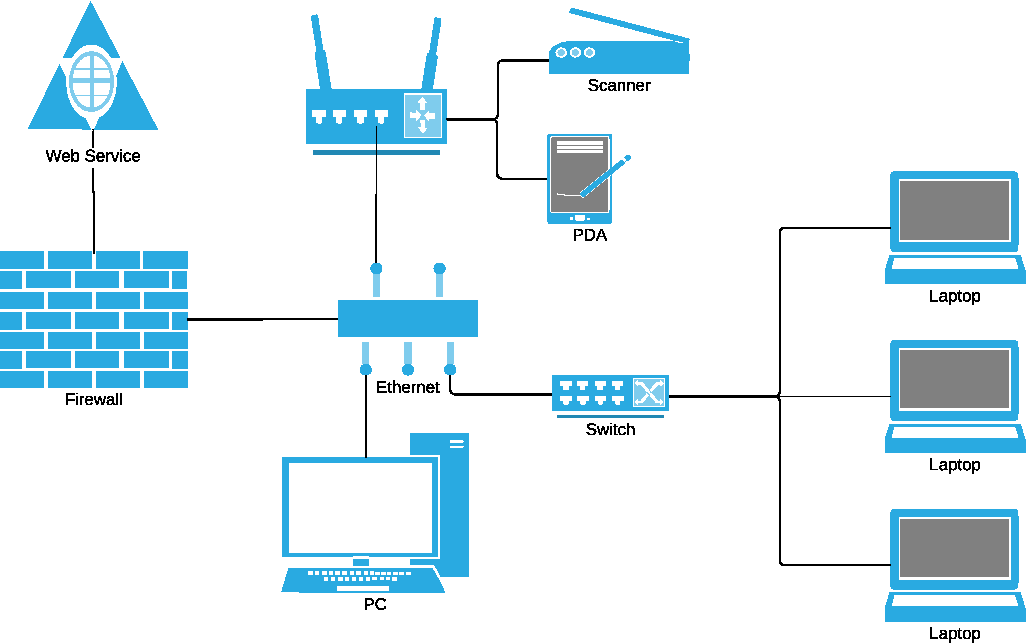
\includegraphics[width=.8\textwidth]{network-color}%
  \end{center}
\end{frame}

\subsection[History]{Past and Future}

\begin{frame}[allowframebreaks=.8]{The History of Internet}
  \begin{description}
  \item[1836:] Telegraph
  \item[1858-66:] Transatlantic cable
  \item[1876:] Telephone
  \item[1957:] USSR launches Sputnik
  \item[1962-68:] \emph{Packet-switching} networks developed
  \item[1969:] Birth of Internet
  \item[1971:] People communicate over a network
  \item[1972:] Computers can connect more freely and easily
  \item[1973:] Global Networking becomes a reality
  \item[1974:] Packets become mode of transfer
  \item[1976:] Networking comes to many
  \item[1977:] E-mail takes off, Internet becomes a reality
  \item[1979:] News Groups born
  \item[1981:] Things start to come together
  \item[1982:] \emph{TCP/IP} defines future communication
  \item[1983:] Internet gets bigger
  \item[1984:] Growth of Internet Continues
  \item[1986:] Power of Internet Realised
  \item[1987:] Commercialisation of Internet Born
  \item[1989:] Large growth in Internet
  \item[1990:] Expansion of Internet continues
  \item[1991:] Modernisation Begins
  \item[1992:] Multimedia changes the face of the Internet
  \item[1993:] The WWW Revolution truly begins
  \item[1994:] Commercialisation begins
  \item[1995:] Commercialisation continues apace
  \item[1996:] Microsoft enters
  \item[1998:] 
\includegraphics[height=.9em]{google}
  \item[Homework:] Meanwhile, what happened in China?
  \end{description}
\end{frame}

\subsection[Internet]{The Internet}

\begin{frame}{What's The Internet?}
  What pops up in your mind if I say ``Internet''?\pause
  
  \begin{iblock}{For me, the answer is...}
    \begin{center}
      
\includegraphics[width=.4\textwidth]{google}%
    \end{center}
      and...\pause
    \begin{center}
      \Tcpip{}%
    \end{center}
  \end{iblock}
\end{frame}


\end{document}

%%% Local Variables:
%%% mode: latex
%%% TeX-master: t
%%% End:
